\newpage
%\pagestyle{empty}

\begin{minipage}[c]{.25\linewidth}
	
\includegraphics[width=4cm]{images/LEnsE_IOGS.jpg}
\end{minipage} \hfill
\begin{minipage}[c]{.4\linewidth}

\begin{center}
\vspace{0.3cm}
{\Large \textsc{Opto-Électronique}}

\medskip

5N-027-SCI \qquad \textbf{\Large TD Séance 2}

\end{center}
\end{minipage}\hfill

%%%%%%%%%%%%%%%%%%%%%%%%%%%%%%%%%%
\section{TD2 - Amplificateur Linéaire Intégré (ALI)}

Aussi appelé \textbf{Amplificateur Opérationnel} (AOP)

%%%%%%%%%%%%%%%%%%%%%%%%%%%%%%%%%%%%%%%%%%%%%%%%%%%%%%%
\subsection{Exercice 1 - Amplificateur linéaire intégré}
On fournit en annexe une partie de la documentation technique de l'amplificateur linéaire intégré (ALI) \textbf{TL081}.

\begin{enumerate}
	\item Cherchez dans la documentation les valeurs des paramètres électriques suivants :
	\begin{enumerate}
		\item Tension d'alimentation (Supply Voltage)
		\item Tension d'entrée différentielle maximale
		\item Amplification différentielle 
		\item Gain unitaire ou produit gain-bande-passante
		\item Impédance d'entrée 
		\item Slew Rate
	\end{enumerate}
	\item Précisez à quoi corresponde chacun de ces paramètres.
	\item Rappelez la relation entre les entrées $V^+$, $V^-$ et la sortie $V_S$ d'un ALI.
	\item Tracez la caractéristique $V_S = f (\varepsilon)$ où $\varepsilon = (V^+ - V^-)$ pour cet ALI avec $V_{CC} = 15\operatorname{V}$.
	\item Est-ce un bon amplificateur ? Quelle est sa bande-passante ?

\end{enumerate}


%%%%%%%%%%%%%%%%%%%%%%%%%%%%%%%%%%%%%%%%%%%%%%%%%%%%%%%
\subsection{Exercice 2 - Montage amplificateur inverseur}
On se propose d'étudier à présent le montage suivant :

\begin{center}
\begin{circuitikz} 
	\node [op amp, fill=blue!10!white](A1) at (0,0){\texttt{AOP1}};
	\draw (A1.-) to[short] ++(-.5,0) coordinate(A) to[short] ++(0,1.5) coordinate(B) to[R=$R_2$] (B -| A1.out) to[short, -*] (A1.out);
	\draw (A1.-) to[short,-*] ++(-.5,0) coordinate(AA) to[R=$R_1$] ++(-2.5,0) coordinate(BB) to[short,-o] ++(-.5,0) coordinate(CC);
	\draw (A1.+) to[short] ++(0,-0.5) node[ground]{};
	\draw (A1.out) to[short,-o] ++(1,0) coordinate(D);
	\draw (-4.6,-1) edge[->,color={green!40!black}] (-4.6,0.3);
	\node[text={green!40!black}] (Ve) at (-5.1,-0.35){$V_e$}; 
	\draw (-4.6,-1.3)  to[open,-o] ++(0,0) node[ground](GND){};
	\draw (2.2,-1) edge[->, color={red}] (2.2,-0.3);
	\node[text={red}] (Vs) at (1.7,-0.6){$V_s$}; 
	\draw (2.2,-1.3)  to[open,-o] ++(0,0) node[ground](GND){};
	
\end{circuitikz}
\end{center}

\begin{enumerate}
	\item Donnez la relation entre $V_S$ et $V_E$ du circuit précédent en utilisant la relation d'entrées-sortie de l'exercice 1.
	\item Quelle hypothèse fait-on souvent lorsqu'on utilise des ALI avec une rétroaction négative ?
	\item Quelle relation trouve-t-on alors entre $V_S$ et $V_E$ en partant de cette hypothèse ?
	\item Cette hypothèse est-elle justifiée ?
\end{enumerate}

\newpage


%%%%%%%%%%%%%%%%%%%%%%%%%%%%%%%%%%%%%%%%%%%%%%%%%%%%%%%
\subsection{Exercice 3 - Mettre en forme un capteur de température}
On se propose d'étudier le circuit suivant :

\begin{center}
	
\includegraphics[width=16cm]{images/capteur_conditionnement.png}
\end{center}

La thermistance utilisée est de type PT100. La relation entre sa résistance (en Ohms) et la température (en \degre{}C) est la suivante :
$$R(T) = 100~(1 + 3.908×10^{-3} T - 5.802×10^{-7} T^2)$$


\begin{enumerate}
	\item Découpez le montage précédent en sous-ensemble.
	\item Donnez la relation de $V_S$ en fonction de $R(T)$ et de $V_Z$. 
\end{enumerate}


%%%%%%%%%%%%%%%%%%%%%%%%%%%%%%%%%%%%%%%%%%%%%%%%%%%%%%%

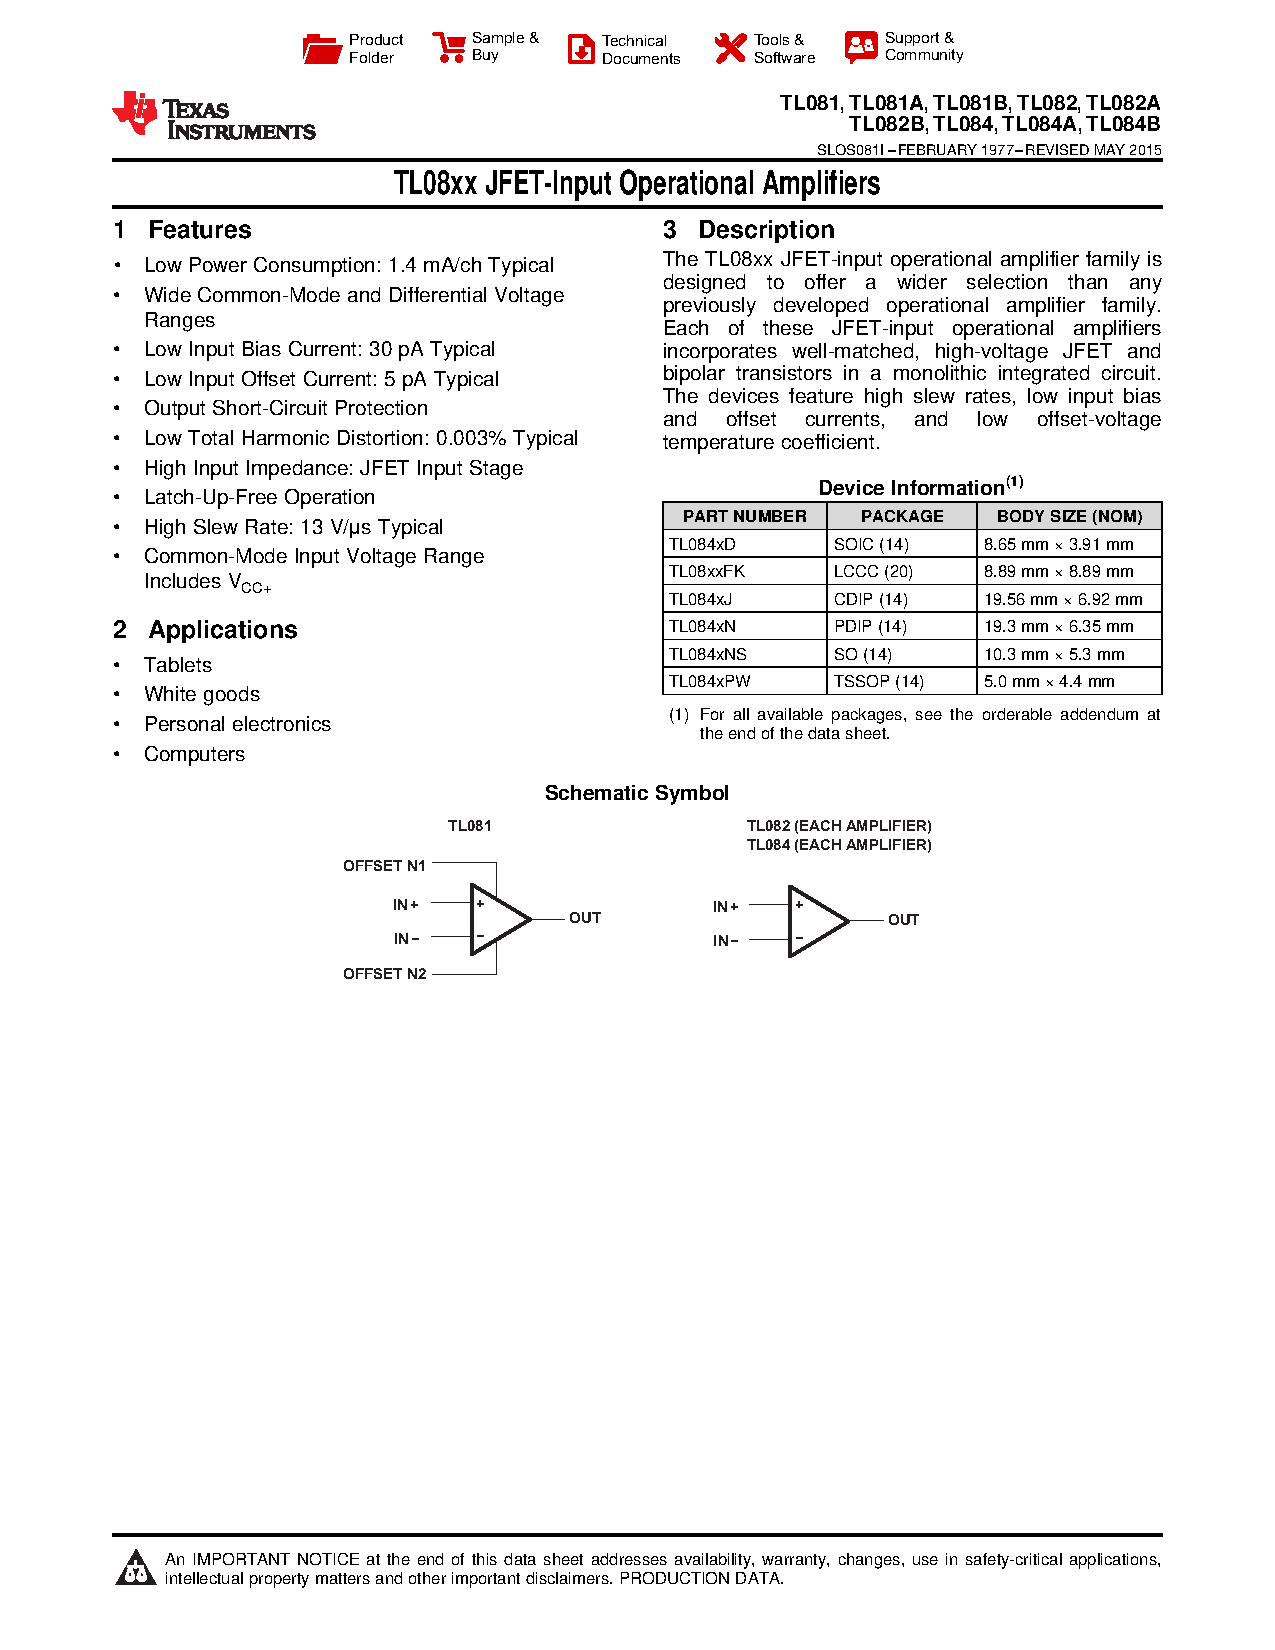
\includepdf[pages=-]{docs/doc_TL071_1p.pdf}

%%%%%%%%%%%%%%%%%%%%%%%%%%%%%%%%%%%%%%%%%%%%%%%%%%%%%%%